% =====================================================================
%  BAB 1 — PENDAHULUAN
% =====================================================================

\chapter{Pendahuluan}

\section{Latar Belakang}
\label{sec:1.1}

Penelitian ini memakai pendekatan \emph{eksperimental} dan \textit{kuantitatif}
dengan \texttt{contoh} kode. Lihat Gambar~\ref{fig:1.alur} dan
Tabel~\ref{tab:1.data} serta Persamaan~\eqref{eq:1.f1} dan Bab~\ref{sec:2.1}.

\begin{figure}[H]
  \centering
  \thesisfigure{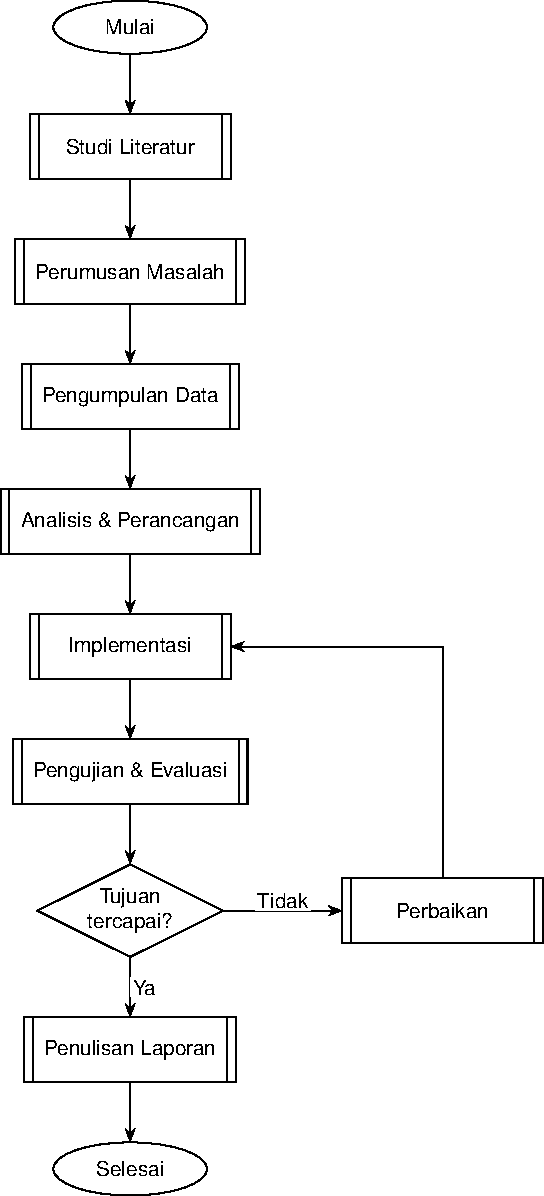
\includegraphics{assets/fig-1.pdf}}
  \caption{Alur penelitian}
  \label{fig:1.alur}
\end{figure}

\section{Rumusan Masalah}
\label{sec:1.2}

Rumusan masalah penelitian adalah sebagai berikut:

\begin{enumerate}
  \item Bagaimana [masalah pertama]?
  \item Bagaimana [masalah kedua]?
\end{enumerate}

\begin{equation}
  F_1 = 2 \cdot \frac{\text{Presisi} \times \text{Recall}}{\text{Presisi} + \text{Recall}}
  \label{eq:1.f1}
\end{equation}

\section{Implementasi}
\label{sec:1.3}

Kode sumber ditunjukkan pada Kode Sumber~\ref{lst:1.kode}.

\begin{lstlisting}[language=Python, caption={Fungsi kunci}, label={lst:1.kode}]
def f(x):
    return x + 1
\end{lstlisting}
